\documentclass[Master]{subfiles}
\begin{document}
\subsection{Numerical Methods and Considerations}
\subsubsection{Diagonalisation}
A second quantisation Hamiltonian is typically written as a sum over creation and anihilation operators. Diagonalising the Hamiltonian in this formulation is numerically non trivial. For a second order Hamiltonian we can use the formalism discussed in \secref{sec:BdG} we bring this Hamiltonian into matrix form.  
$$
\hat{H} = \frac{1}{2}\bra{\vec{\Psi_c}}M\ket{\vec{\Psi_c}} + tr(A)
$$
In order to diagonalise the Hamiltonian $\hat{H}$ we have to diagonalise the matrix $M$, where the eigenvalues give us the excitation energy and the eigen-vectors $\vec{V}_i$ give us the Bogoliubov transformed operators as:
$$ \hat{d}_i = \vec{V}_i^{\dag}\ket{\vec{\Psi}} ; \hat{d}^{\dag}_i = \vec{W}_i^{\dag}\ket{\vec{\Psi}} $$
We are left with the diagonalised Hamiltonian 
$$ \hat{H} = \sum_i \omega_i \hat{d_i}^{\dag}\hat{d_i}$$
Matrix diagonalisation is a standard numerical problem for which several widely-used methods exist. The most common of which are 
the QR Algorithm and the more modern Divide and Conquer algorithm.
\paragraph {QR-Algorithm}
The \textit{QR-algorithm} works based on the \textit{QR-decomposition}: Any $M \in \mathbb{C}^{n\times n}$ matrix can be decomposed into a product of $Q\ R$ where $Q$ is a unitary matrix and $R$ is an upper triangular matrix with $Q$ holding the orthonormalised column vectors of $M$. Conceptually, $R$ containes the projection of a column vector from $M$ and a column vector from $Q$:
$$ M = QR \Leftrightarrow  Q^{\dag}M = R  \Leftrightarrow \braket{Q_i}{M_j} = R_{i,j}$$ 
In practice, $Q$ and $R$ are commonly computed with with householder reflections in  $\mathcal{O}(n^3)$ steps. Doing so with Gram Schmidt is numerically unstable. 
As $Q$ is unitary it can be used as a similarity transformation from $A ~ Q^{\dag}A Q \forall A$.
We can thus define an iteration for $M_n = Q_n R_n$
$$ M_{n+1} = Q_n^{\dag}M_n Q_n = Q_n^{\dag}Q_n R_n Q_n  =  R_n Q_n $$ 
Where $\forall i,j \ M_i \sim M_j$. Thus, when we begin with $M_0 = M$ the eigenvalues of any $M_i$ are the same as the eigenvalues of $M$. However,it can be demonstrated that the matrix entries of $M_i$ below the diagonal vanish with decreasing iterations \cite{bai1989block}. The $M_i$ converges to Hessenberg form.
The algorithm has the following structure:
\begin{algorithm}[H]
\caption{QR-Algorithm}\label{num:QR}
\begin{algorithmic}[1]
\Procedure{}{}
\While{$|A|_{low} > \epsilon$} \Comment{Threshold for lower triangular entries}
\State $Q,R \gets QR(A)$ \Comment{\textit{QR-decompose}}
\State $A \gets R \cdot Q$
\EndWhile
\State $\lambda_i \gets A_{i,i}$ \Comment{Read Eigenvalues from Diagonal}
\EndProcedure
\end{algorithmic}
\end{algorithm}
This method converges well when the eigenvalues are ordered and well spaced.
$$\forall i,j : i < j : |\lambda_i| << |\lambda_j|$$
However, two problems can arise: Degeneracies and eigenvalues with similar magnitude but different phase. The latter can be solved with so-called shifts \cite{bai1989block}. Given a matrix $M$ we can shift the matrix by some constant $c \in \mathbb{C} : M \rightarrow M + c \mathbb{1}$. As 
$Q^{\dag} ( M + c \mathbb{1} )Q = Q^{\dag} M Q+ c \mathbb{1} = R Q+ c \mathbb{1}$ The matrix can be shifted prior to the QR-decomposition and shifted back afterwards. The shift offsets the eigenvalues and can thus separate eigenvalues with similar magnitude. The amplitude of the shift can be fixed or altered each iteration. 
\begin{algorithm}[H]
\caption{QR-Algorithm with Shifts}\label{num:QRShift}
\begin{algorithmic}[1]
\Procedure{}{}
\While{$|A|_{low} > \epsilon$} \Comment{Threshold for lower triangular entries}
\State Determine $c$ 
\State $Q,R \gets QR(A + c \mathbb{1})$ \Comment{\textit{QR-decompose}}
\State $A \gets R \cdot Q - c \mathbb{1}$
\EndWhile
\State $\lambda_i \gets A_{i,i}$ \Comment{Read Eigenvalues from Diagonal}
\EndProcedure
\end{algorithmic}
\end{algorithm}

An even more modern approach is to multiply two shifts together \cite{braman2002multishift}:
$$P = (M + c_1 \mathbb{1})(c_2 \mathbb{1}) = M^2 + (c_1+c_2) M + c_1 c_2 \mathbb{1}$$
We iterate the QR-Decomposition and swapped multiplication of P:
$$Q^{\dag} ( M^2 + (c_1+c_2) M + c_1 c_2) Q = Q^{\dag} M^2 Q + (c_1+c_2) Q^{\dag} M Q+ c_1 c_2 \mathbb{1} =  R Q R Q + (c_1+c_2) R Q+ c_1 c_2 \mathbb{1}$$
We abort the iteration when the lower triangular entries of $P$ have become sufficiently small.
The eigenvalues are retrieved from the product $P_n$ by finding the roots of a set of $N$ quadratic equations:
$$
 \lambda_i^2 + (c_1+c_2)\lambda_i + c_1 c_2 = P_{i,i}
$$

\begin{algorithm}[H]
\caption{QR-Algorithm with two Shifts}\label{num:QRShift2}
\begin{algorithmic}[1]
\Procedure{}{}
\State Determine $c_1,c_2$
\State $P \gets (A^2 + (c_1+c_2)A + c_1 c_2 \mathbb{1})$
\While{$|P|_{low} > \epsilon$} \Comment{Threshold for lower triangular entries}
\State $Q,R \gets QR(P)$ \Comment{\textit{QR-decompose}}
\State $P \gets R \cdot Q$
\EndWhile
\State solve $\lambda_i^2 + (c_1+c_2)\lambda_i + c_1 c_2 = P_{i,i}$ \Comment{find all N Eigenvalues} 
\EndProcedure
\end{algorithmic}
\end{algorithm}
This can be done with an arbitrary number of shifts as for every monimial $Q^{\dag}(QR)^k Q = (RQ)^k$ Thus, for any polynomial of arbitrary degree $Q^{\dag}PQ \sim P$. However, when using higher order polynomials they need to be solved numerically as no analytical solutions exist.

\paragraph {Divide and Conquer}
While very stable and well tested versions of the \textit{QR-algorithm} exist it does not lend itself easily to parallelisation. Contrarily, the \textit{Divide and Conquer algorithm} \cite{cuppen1980divide} is very efficient for parallel architectures and even Graphics Processing Units (GPUs). The goal is to split the problem of diagonalising a matrix $A$ into the problem of diagonalising two matrices $A^{\uparrow}$ and $A^{\downarrow}$. This is the so called \textbf{Divide} step. It can, theoretically, be repeated until the matrix is of size 1 where the eigenvalue is trivial. In practice, however, most implementations use the \textit{QR-algorithm} once sufficiently many small $a$ matrices exit, to balance the workload between multiple threads. 
The resulting eigenvalues of  $A^{\uparrow}$ and $A^{\downarrow}$ are then used to calculate the eigenvalues of $A$ in the \textbf{Conquer} step. This step has to be repeated until the eigenvalues of the full matrix are known. \\
Many modern implementations of the \textit{QR-algorithm} already use this method when the matrix happens to approximate a block matrix of the form$\left( \begin{array}{c|c}
     A & B \\
     \hline
     0 & C
\end{array}\right)$. In this scenario it is sufficient to \textbf{Divide} by simply diagonalising only the matrix blocks $A,C$, then the \textbf{Conquer} step is trivial as the eigenvalues of $M$ are just the union of the eigenvalues of $A$ and $C$. When parallelising, this is only of limited benefit as the \textbf{Divide}-step occurs non deterministically. Instead, we wish to perform a \textbf{Divide} at the start. The so called divide and conquer algorithm begins with a preparation step.
The matrix is brought to tridiagonal form with householder transformations. 
In the \textbf{Divide}-step \cite{cuppen1980divide}, the matrix is then split into blocks. The remaining off diagonal elements $b$ are treated as a rank-1 modification.
$$ M = 
\left(\begin{array}{c|c}
    A^{\uparrow} & 0 \\
    \hline
   0  & A^{\downarrow}
\end{array}\right)
+ b\left( \begin{array}{cc|cc}
     &&& \\
      &  1&1&\\
     \hline
     &1&1&  \\
     & &&
\end{array}\right) = \left(\begin{array}{c|c}
    A^{\uparrow} & 0 \\
    \hline
   0  & A^{\downarrow}
\end{array}\right) + b  \vec{w}\vec{w}^T
$$
With $\vec{w} = \delta_i$ one at the cut line and zero everywhere else.
Contrary to the simple case above here the \textbf{Conquer}-step is nontrivial because of the rank-1 modification.
$$
\left(\begin{array}{c|c}
    T_1 &  \\
    \hline
     & T_2
\end{array}\right)\left(
\left(\begin{array}{c|c}
    D_1 &  \\
    \hline
    & D_2
\end{array}\right)
+ 2b \ \vec{z}\vec{z}^T\right)
\left(\begin{array}{c|c}
    T_1 &  \\
    \hline
     & T_2
\end{array}\right)^T
= M
$$
$$
\vec{z}= \frac{1}{\sqrt{2}}\left(\begin{array}{c|c}
    T_1 &  \\
    \hline
    & T_2
\end{array}\right)^T \vec{w} = \frac{1}{\sqrt{2}}\left(\begin{array}{c}
    \vec{T_1}^{lr}  \\
    \hline
     \vec{T_2}^{fr}
\end{array}\right)^T
$$
with $\vec{T_1}^{lr}$ the last row of $T_1$ and $\vec{T_2}^{fr}$ the first row of $T_2$.
It can be further shown \cite{cuppen1980divide} that  is equivalent to finding the solutions of:
$$1 + b \sum_{i} \frac{\vec{z}_i ^2}{D_{i,i} - \lambda} = 0$$
A recursive implemention has the following form.
\begin{algorithm}
\caption{Divide and Conquer}\label{num:DivNConq}
\begin{algorithmic}[1]
\State Bring $A$ to tridiagonal form
\State Divide(A)
\Procedure{Divide}{A}
\If {Divided enough} \Comment{Suffitiently many matrices for parallelisation}
\State Divide $A$ in $A^{\uparrow},A^{\downarrow}$ and $b$ 
\State \Return{Conquer(Divide($A^{\uparrow}$), Divide($A^{\downarrow}$),$b$)} 
\Else {}
\State \Return {QR(A)}
\EndIf
\EndProcedure
\Procedure{Conquer}{$A^{\uparrow},A^{\downarrow},b$}
\State Solve the Polynomial $1 + b\sum_{i} \frac{\vec{z}_i ^2}{D_{i,i} - \lambda}$ \Comment{e.g. with Newton-Raphson}
\EndProcedure
\end{algorithmic}
\end{algorithm}
\subsubsection{Optimisation}
\paragraph{Gradient Descent}\label{num:GD}
A simple optimization method is a backtracking \textit{Gradient descent}.
The basic idea of \textit{Gradient descent} is to iterative take steps in the direction of steepest descent, thus in the opposite direction of the gradient.
$$ \vec{x}_{i+1}= -\lambda \nabla Err(\vec{x}_{i+1})$$
A \textit{Backtracking Gradient descent} attempts to automatically adjust the learning rate $\lambda$.
It only attempts a step against the gradient but before the step is accepted the error before and after the step are compared. If the error failed to decrease, the learning rate is divided by two and a new attempt is made. If the step is accepted the learning rate is reset to its initial value. Once a desired accuracy is reached $\lambda < \epsilon$ iteration is aborted.
\begin{algorithm}
\caption{Back stepping Gradient Descent}\label{FGradDescent}
\begin{algorithmic}[1]
\Procedure{}{}
\State $\lambda \gets 10$
\State  $\Theta \gets (0,0,\pi/2)$
\Loop
\State $Err_{Old} \gets Err(\Theta)$
\While {$Err_{Old} < Err(\Theta - \lambda \nabla Err)$}
\State $\lambda \gets \lambda/2$
\If {$\lambda < \epsilon$}
\State break
\EndIf
\EndWhile
\State $\Theta \gets \Theta - \lambda \nabla Err$
\EndLoop
\EndProcedure
\end{algorithmic}
\end{algorithm}
This method is guaranteed to converge for convex functions.
\paragraph{Programmatic Differentiation}
The numerical optimisation methods described all require the derivatives of the function. As the degrees of freedom grow, programmatic evaluation of derivative is becomes necessary. Several approaches to programmatic differentiation exist.
\textit{Symbolic differentiation} uses a set of rules to determine the derivative similar to how a human would compute the derivative. This is slow, however, and is not guaranteed to succeed.
\textit{Numerical differentiation} approximates the Cauchy form of the derivative numerically
$$
f'(x) = \lim_{h \rightarrow 0} \frac{f(x+h)-f(x)}{h} 
$$
However, this can become unstable for small numbers.
A modern approach is \textit{Auto differentiation} \cite{rall1981automatic}. The basic idea is to use the chain rule to compute the derivative from the derivatives of all sub functions involved. 
It is especially efficient when both the value and derivative are required and also helps with storing and handling derivatives. In practice auto differentiation uses three concepts:
\begin{itemize}\label{num:autodiff}
    \item Forward or backward propagation:\\
    The formula is translated into a tree. Derivatives are calculated and accumulated according to the chain rule: $\frac{d \ f(g(x))}{dx} = f'(g(x)) g'(x)$\\
    \item Symbolic differentiation:\\
    Where the derivative of a function is known e.g. $sin(x)$ the known derivative is used (e.g. $cos(x)$)\\
    \item Infinitesimal algebra
\end{itemize}

An elegant way to do this is to use the smooth infinitesimal analysis \cite{bell1988infinitesimals} \cite{grunwald1906duale}. This method is commonly used to compute derivatives in Machine Learning.
The field $\mathbb{K}$ is extended with the new element $\epsilon$ to the psudofield of dual numbers $\mathbb{\kappa} = \{x+y\epsilon, x,y \in \mathbb{F}\}$. The algebra has the following form:
\begin{table}[H]
    \centering
    \begin{tabular}{c|cc}
         &$1$ & $\epsilon$\\
         \hline
         $1$&$1$ &$ \epsilon$\\
        $\epsilon$ & $\epsilon$&$0$
    \end{tabular}
    \caption{The Infinitessimal Algebra}
    \label{tab:my_label}
\end{table}
This new pseudo field fullfilles all field Axioms besides $\epsilon$ having no multiplicative inverse. However, an operator $\forall x,y \in \mathbb{\kappa} : \mathfrak{E}(x+y\epsilon) = y$ can be defined. This subtle difference is important. As $ \forall x,y \in \mathbb{\kappa} \ \mathfrak{E}(x)\mathfrak{E}(y)$ is well defined while $\frac{x}{\epsilon}\frac{y}{\epsilon} = \frac{xy}{\underbrace{\epsilon^2}_{=0}}$ is not!\\ Analogous a "normal part" operator $\forall x,y \in \mathbb{\kappa} : \mathfrak{N}(x+y\epsilon) = x$ can be defined. Generally, an inverse exists exactly when the normal part is non zero.
$$
\forall x \in \mathbb{K} \left(\exists y \in \mathbb{K} : x y = \mathbb{1} \iff \mathfrak{N}(x)\neq 0 \right)
$$
The following identity can be proven using category theory\cite{bell1988infinitesimals}:
$$\forall x,y \in \mathbb{R} : f(x+y\epsilon) = f(x)+ f'(x)y \epsilon$$
$$\Rightarrow f'(x) = \mathfrak{E}(f(x+\epsilon))$$
To illustrate:
$$
(x+\epsilon)^n = \sum_k^n \binom{k}{n} x^{n-k} \epsilon^k = x^n + x^{n-1}\epsilon 
$$
Further all common derivation rules hold:
\begin{center}
Sum Rule
$$ \frac{d}{dx} (f(x)+g(x)) = \mathfrak{E}(f(x+\epsilon) + g(x+\epsilon)) = \mathfrak{E}(f(x+\epsilon)) + \mathfrak{E}(g(x+\epsilon)) = f'(x)+g'(x)$$
Product Rule:
$$ \frac{d}{dx} (f(x)g(x)) = \mathfrak{E}(f(x+\epsilon)  g(x+\epsilon)) = \mathfrak{E}((f(x)+f'(x) \epsilon)(g(x)+g'(x)\epsilon)) 
$$
$$=\mathfrak{E}((f(x)g(x) +f'(x)g(x) \epsilon+f(x)g'(x)\epsilon + f'(x)g'(x)\underbrace{\epsilon^2}_{=0})) = f'(x)g(x)+f(x)g'(x)$$
Chain Rule :
$$ \frac{d}{dx} f(g(x)) = \mathfrak{E}(f(g(x+\epsilon))) = \mathfrak{E}(f(g(x)+g'(x)+\epsilon))  =
\mathfrak{E}(f(g(x))+f'(g(x))g'(x)\epsilon)=f'(g(x))g'(x)$$
\end{center}
Similar to the complex number aglebra the infinitesimal algebra is simple to implement on a computer. Thus, auto differentiation is a stable and fast way to compute derivatives. This is especially efficient for algebra, where most operations like matrix and vector products are based on large numbers of elementary additions and multiplications.

\paragraph{Broyden–Fletcher–Goldfarb–Shanno Method} \label{num:BFGS}
The \textit{Broyden–Fletcher–Goldfarb–Shanno} (BFGS) method \cite{broyden1970convergence}\cite{fletcher1970new}\cite{goldfrab1970family}\cite{schanno1970conditions} is an advanced numerical optimisation method.
Contrary to Newtons method:
$$
\vec{x}_{k+1} = \vec{x}_k - (\mathbf{H}_f)^{-1}*\nabla f
$$
The BFGS method only approximates the calculating and inverting the Hessian $(\mathbf{H}_f)^{-1}$. Thus, avoiding the  computational complexity of matrix inversion  $\mathcal{O}(n^3)$ reducing the BFGS method to  $\mathcal{O}(n^2)$.
$$
\vec{x}_{k+1} = \vec{x}_k \underbrace{- B_k^{-1} *\nabla f}_{= \vec{s}_k}
$$
Where $B_k^{-1}$ is the approximate inverse Hessian. $B_k^{-1}$ is iterated as:

$$
B_{k+1}^{-1} = B_k^{-1} + \frac{(\vec{s}_k^T \vec{y}_k + \vec{y}_k^T B_k^{-1}\vec{y}_k )\vec{s}_k^T\vec{s}_k}{( \vec{s}_k^T\vec{y}_k)^2} - \frac{ B_k^{-1} \vec{y}_k\vec{s}_k^T+ \vec{s}_k\vec{y}_k^T B_k^{-1} }{\vec{s}_k^T\vec{y}_k}
$$
$$
\vec{y}_{k} = \nabla f(\vec{x}_{k+1}) - \nabla f(\vec{x}_k)
$$


\begin{algorithm}
\caption{BGFS}\label{BGFSAlg}
\begin{algorithmic}[1]
\State guess initial $\vec{x}_0$ and $B_0^{-1}$ 
\Procedure{}{}
\While{$|\nabla f(\vec{y}_k)| > \epsilon$}
\State $\vec{p}_k \gets \vec{x}_k - B_k^{-1} *\nabla f$ \Comment{find direction}
\State $\alpha_k \gets arg \  min f(\vec{x}_k + \vec{p}_k) $ \Comment{perform line search}
\State $\vec{s}_k \gets \alpha_k \vec{p}_k$
\State $\vec{x}_{k+1} \gets \vec{x}_k +\vec{s_k}$ \Comment{update $x$}
\State $\vec{y}_{k} \gets \nabla f(\vec{x}_{k+1}) - \nabla f(\vec{x}_k)$
\State $B_{k+1}^{-1} \gets B_k^{-1} + \frac{(\vec{s}_k^T \vec{y}_k + \vec{y}_k^T B_k^{-1}\vec{y}_k )\vec{s}_k^T\vec{s}_k}{( \vec{s}_k^T\vec{y}_k)^2} - \frac{ B_k^{-1} \vec{y}_k\vec{s}_k^T+ \vec{s}_k\vec{y}_k^T B_k^{-1} }{\vec{s}_k^T\vec{y}_k}$ \Comment{update  $B^{-1}$}
\EndWhile
\EndProcedure
\end{algorithmic}
\end{algorithm}

\subsubsection{Time Evolution}

\paragraph {ODE-solving / Initial Value Problem}
$$
f'(x) = g(x,f(x))
$$
Given an ordinary differential equation (ODE) and an initial value $f(0)=x$ the  simplest imaginable way to solve the ODE numerically is to discretise $x$ in steps of step size $h$ and iterate:
$$
f_{n+1} = f_n + h g(x_n,f_n)
$$ 
This is crude approach is known as \textit{Forward Euler}. When trying to solve an ODE as simple as $f' = x$ the method is inaccurate: It grows slower than the exact solution. This is because the derivative is monotonous growing in $x$ and the method only evaluates the derivative at the start of the interval $[x_n,x_n+h]$. A simple improvement would be to evaluate the derivative at $x_n+ h/2$ this is referred to as the \textit{Midpoint Method}.
However, in general one would need to know $f(x_n+ h/2)$ to do that. So two approaches are possible:
\begin{itemize}
    \item \textit{Explicit Midpoint method}\\
    Use \textit{Forward Euler} to compute $f(x_n+ h/2)$ then calculate $f'(x_n+ h/2)$ to compute $f_{n+1}$ Thus iterate:
    \begin{dmath} \label{num:midpoint}
    f_{n+1} = f_n + h g(x_n +\frac{h}{2}, f_n + \frac{h}{2} g(x_n,f_n))
    \end{dmath}
    \item \textit{Implicit Midpoint method}\\
    While one can not iterate:
    $$f_{n+1}= f_n + h g(x_n +\frac{h}{2}, \frac{f_n+f_{n+1}}{2})$$
    as $f_{n+1}$ appears on both sides and the equation can in general not be seperated.
    The equation can be solved numerically for $f_{n+1}$. Thus, a self-consistent solution is approximated this is called an implicit method.
\end{itemize}
\paragraph{Runge Kutta Schemes}
The most-widely used method is RK4 \cite{runge1895numerische}
$$f_{n+1} = f_n + \frac{h}{6} (k_1 + 2k_2 + 2k_3 + k_4)$$
With:
$$k_1=g(x_n,f_n)$$
$$k_2=g(x_n + \frac{h}{2},f_n+\frac{h}{2}k_1 )$$
$$k_3=g(x_n+\frac{h}{2},f_n +\frac{h}{2}k_2)$$
$$k_4=g(x_n+h,f_n+ h k_3)$$
Here four steps are used to sample the deviate in the interval $[x_n,x_n+h]$ with different approximations for $f(x)$ in the interval. It is intuitively clear that with more steps, a higher degree of accuracy can be reached, in principle.
A general scheme can be stored in Butcher tableaus \cite{butcher1987numerical}.
$$
    \begin{array}{c|c}
        \vec{c} & A\\
         \hline
         & \vec{b}^T
    \end{array}
$$
With $c,b \in \mathbb{R}^n$ and $A \in \mathbb{R}^{n \times n}$ where n is the order or number of steps of the method.
The $\vec{c}$ vector stores the $x$ sampling points, the $\vec{b}$ vector stores the weights and the matrix A describes how $f(x)$ is sampled.
\mypagebreak
For an explicit method $A$ is a lower triangular matrix and for an implicit method $A$ contains no zero elements on the upper triangular side.
The recursion is then:
$$
f_{n+1} = f_n + h \sum_j b_j k_j
$$
$$
k_j = g(x_n+h c_j, f_n + \sum_j a_j k_j)
$$
\begin{table}[H]
    \centering
    \begin{tabular}{c|cccc}
        $0$& & & &  \\
         $\frac{1}{2}$&$\frac{1}{2}$ & & &  \\
         $\frac{1}{2}$&$0$& $\frac{1}{2}$& &  \\
        $1$&$0$&$0$&$1$&  \\
         \hline
         & $\frac{1}{6}$&$\frac{1}{3}$ &$\frac{1}{3}$ & $\frac{1}{6}$
    \end{tabular}
    \caption{RK4 Butcher tableau}
\end{table}
Other common Runge-Kutta methods are Dormand–Prince\cite{DORMAND198019} and Fehlberg \cite{fehlberg1968classical}
\paragraph {A-stability}
Mathematically, a reasonable method must converge towards the exact solution in the limit $\Delta x \rightarrow 0$; however, in practice, we can only get to small $\Delta x$ as compute time goes to infinity and, even more importantly, accuracy decreases in practice. As computers store numbers with a fixed precision rounding errors occur. By summing up more and more terms this error increases.
The accuracy of a method for a given $\Delta x$ is not generally easy to compute as it depends on the specific ODE and initial value. However, the stability of the method can be computed. In contrast to convergence and accuracy the stability only predicts if the method does not diverge towards $\pm \infty$. 
In the pathological case a numerical method can be either accurate or stable but not both for example $f(x)=e^x; f'(x) = f(x)$, as here the exact solution diverges itself. However, when the ODE is bounded $g_{max} < |g(x,f)|; \Re{g(x,f)} < 0$ stability is useful as it guarantees non divergence for small enough $\Delta x$.
The region in the complex plane where a given method is stable for $g_{max}*\Delta x$ is called region of stability.
Explicit methods have a limited region of stability \figref{fig:RK-AStabRegion}.
\begin{figure}[H]
    \centering
    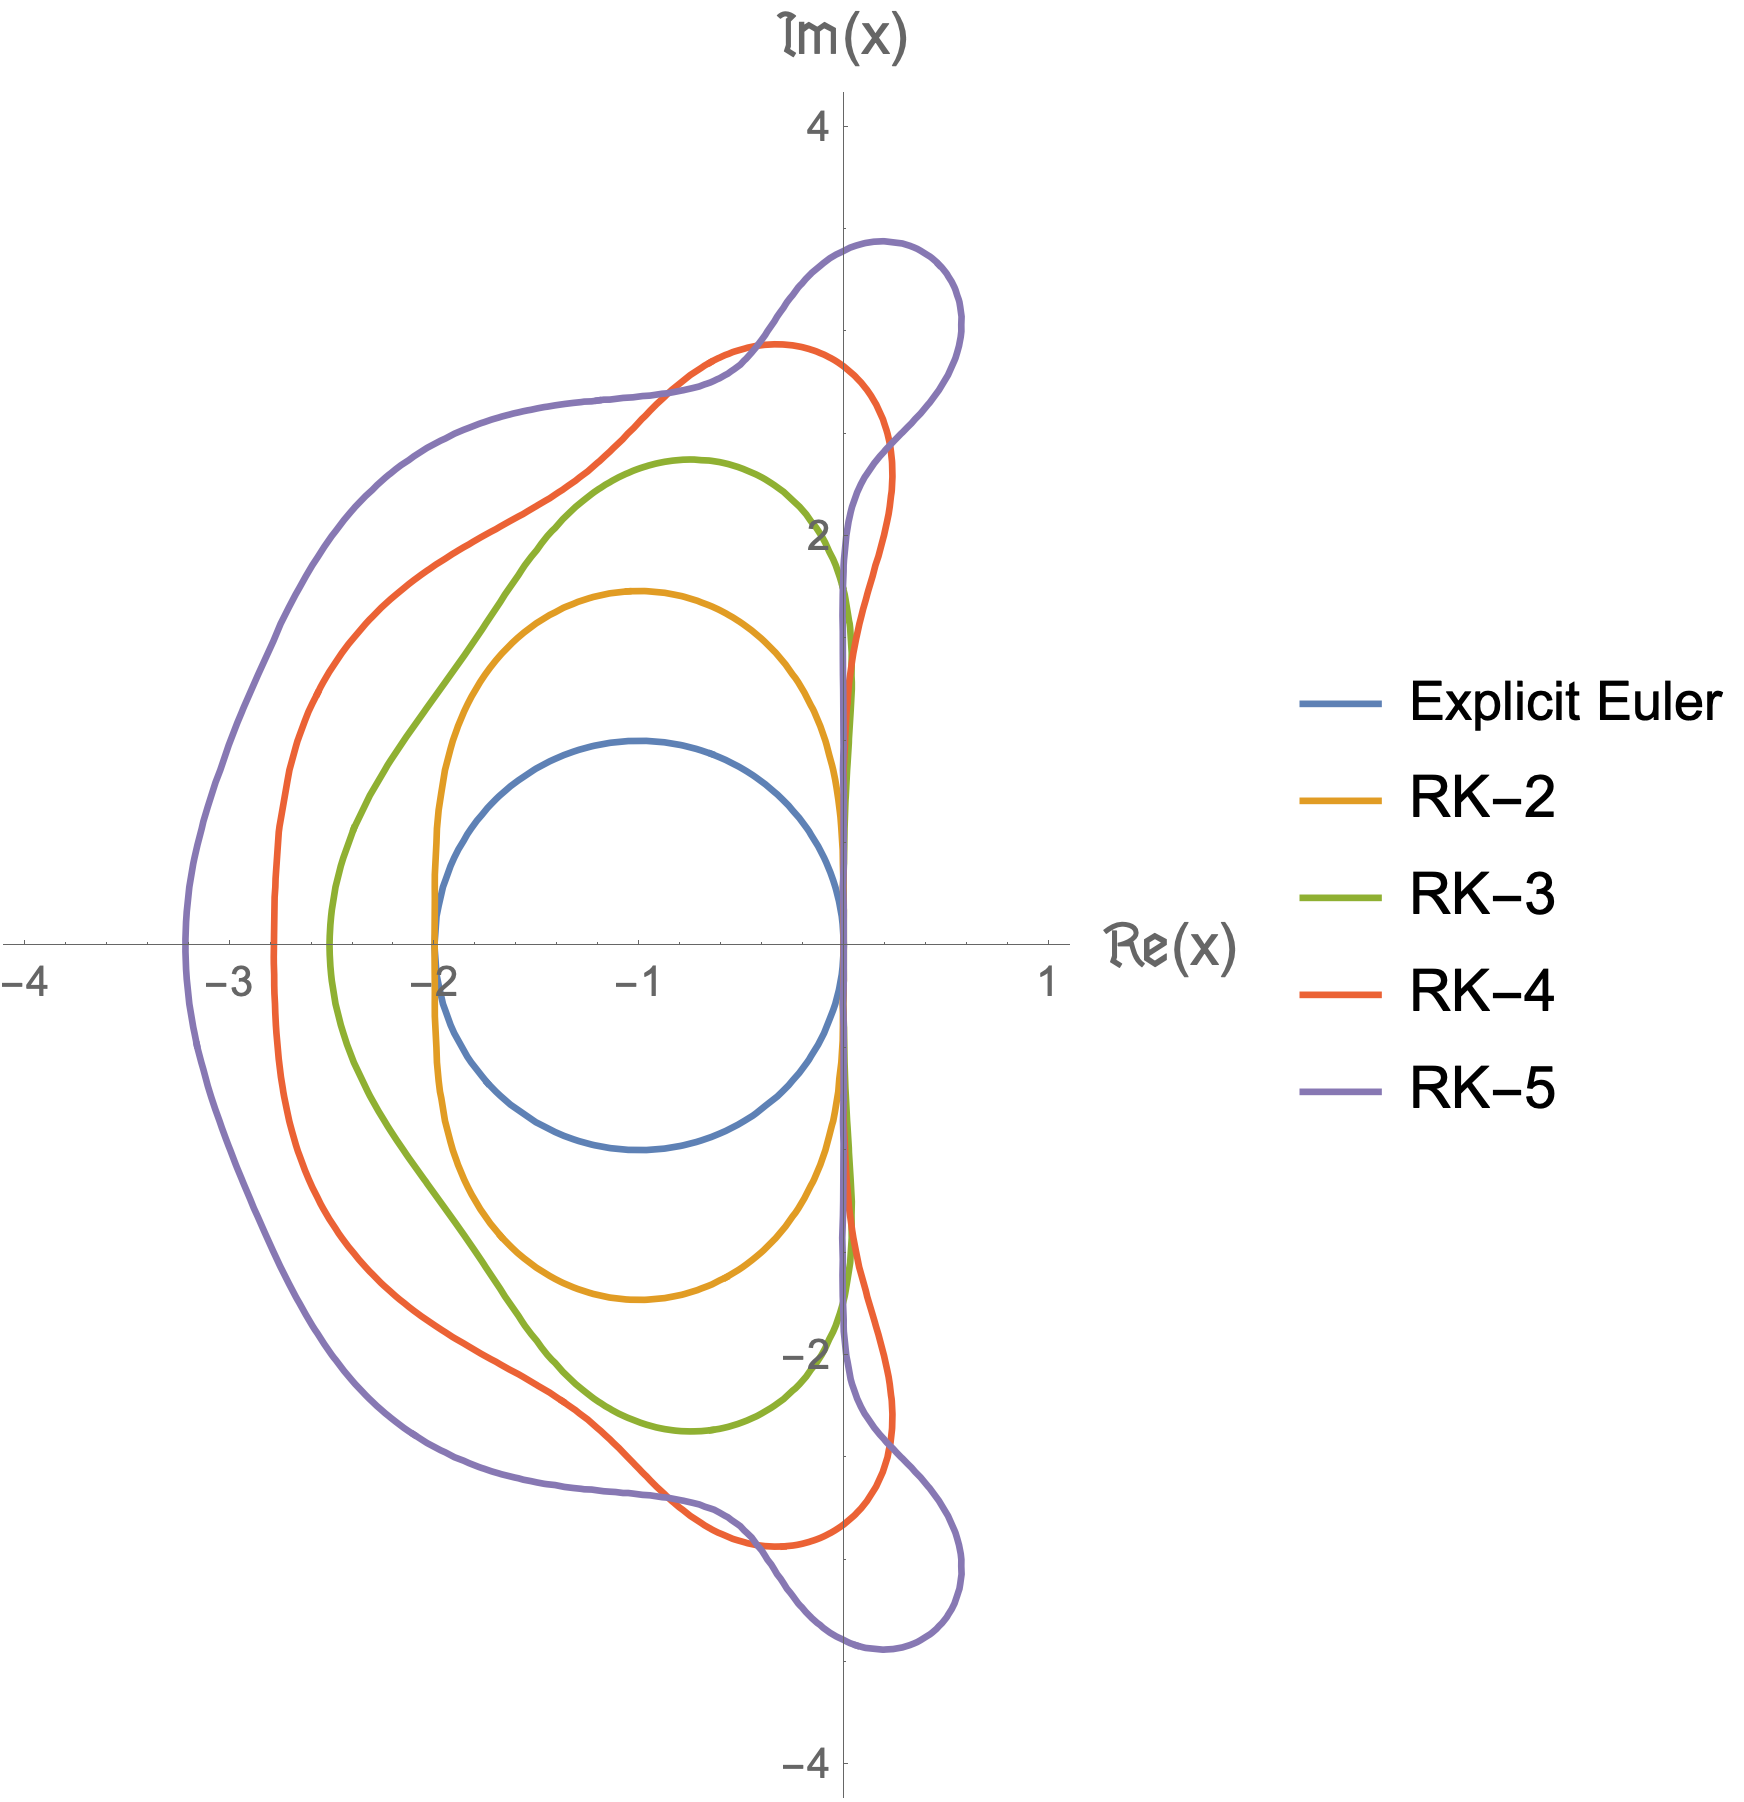
\includegraphics[width=0.6\linewidth]{imgs/StabilityRegion.png}
    \caption{Outline of the Stability Regions for explicit Euler and Runge-Kutta schemes of orders 2,3,4,5}
    \label{fig:RK-AStabRegion}
\end{figure}
In practice this provides an upper limit on the step size and a larger derivative corresponds to smaller step sizes. For implicit solvers, it is possible to generate schemes that are stable for all $|h g_max|-1 > 1$ thus explicitly L-Stable.
\paragraph {Error Estimation / Automatic Step Size}
For many problems, choosing a constant step size according to a global limit $\forall x,f :g_max \geq |g(x,f)|$ may be inefficient. A more efficient way is to change the step size dynamically. When an error approximation or limit exists, a method can adjust the step size.

\paragraph {Stiffness}
Given the following ODE:
$$
\dot{\vec{v}} = M \vec{v}
$$
When one eigenvalue of $M$ is very large and one is small, solving the ODE becomes hard with simple methods as the large eigenvalue forces a small step size even when the behaviour is dominated by the small eigenvalue. The behaviour can be classified by the stiffness ratio. For an ODE:
$$
\dot{\vec{v}} = M \vec{v} + f(t)
$$
with a diagonalisable $M$ and all eigenvalues on the left side of the complex plane $\forall i: \Re{\lambda_i} < 0$.
The stiffness ratio $\eta_{stiff}$ is:
$$
\eta_{stiff} = \frac{\max_i |\Re{\lambda_i|}} {\min_i  |\Re{\lambda_i|}}
$$
The stiffness ratio gives the worst case efficiency for the step size.
A problem is considered stiff if $\eta >> 1$,
and in this instance we have a similar consideration for an oscillatory system:
$$
\dot{\vec{v}} =  -\frac{i}{\hbar}H \vec{v}
$$ 
with $H$ hermitian. Thus, all diagonals are real $h_{k,k} \in \mathbb{R}$. According to the definition above, this system is not stiff. The exact solution for an eigenvector $ H \vec{v} = \lambda \vec{v}$ is:
$$\vec{v}(t) =  \exp(-\frac{i}{\hbar} \lambda) \vec{v}  = (\cos(-\frac{i}{\hbar} \lambda) + i \sin(-\frac{i}{\hbar} \lambda))\vec{v}$$
In regard to the Nyquist–Shannon sampling theorem \cite{shannon1949communication} the step size has to be smaller than:
$$\Delta t <  \frac{\hbar}{4 \pi \lambda_{max}}$$ 
Even when one has an initial vector $\vec{v}(0)$ numerically close to an eigenvector, one needs to reduce the step size for $\lambda_{max}$. As the numerical vector will have some small numerical error $\vec{v} = \vec{v}_{\parallel}+\vec{v}_{\bot}$ where $\vec{v}_{\parallel}$ is the exact part and $\vec{v}_{\bot}$ is the error. In general $|\braket{\vec{v}_{\bot}}{\vec{v}_{max}}|> 0$
Even when one ignores the numerical overlap with a $\ket{\vec{v}_{max}}$ and the resulting high-frequency oscillations as numerical errors they can lead to numerical instability. Most higher order (>2) methods have an a-stable interval(s) on or bounded by the imaginary axis.
Then, the numerical overlap $\vec{v}_{\bot}$ can diverge thus $|\vec{v}_{\bot}| \rightarrow \pm \inf$ while the  $|\vec{v}_{\parallel}| = \textit{const}$, thus the entire solution becomes unstable. Therefore, the modified stiffness ratio is used.
\begin{dmath}\label{num:modStiffRatio}
\eta_{osc} = \frac{\max_i|\Im{\lambda_i|}} {\min_i|\Im{\lambda_i|}} = \frac{E_{amax}}{E_{amin}}
\end{dmath}
In the context of the Schrodinger equation, this becomes a fraction of physical energies with the largest and smallest absolute value. $E_{amax} = \max_i|E_i|; E_{amin} = min_i|E_i|; $ This is problematic for a system with states close to zero. As the step size can be come arbitrarily inefficient. Both implicit and automatic step size methods can be used to attempt calculations with large $\Delta t$. For a physical system this means that while an energy shift can reduce the modified stiffness ratio to an arbitrary value, this decreases the maximal step size further as the shift increases $E_{max}$. The infinite stiffness ratio is due to the fact that for an exact constant zero energy mode the solution is trivial. However, the modified stiffness ratio ignores the fact that for a time dependent $M(t)$, the instantaneous zero energy mode need not be constant $\partial_t \ket{\phi_o} \neq 0$. Such a mode is no solution to the  Schröedinger equation. E.g.:
$$
M = R(-t)\left(
\begin{array}{cc}
 1 & 0 \\
 0 & 0 \\
\end{array}
\right)R(t)
$$
With $R(t)$ the 2D rotational matrix:
$$
R(\alpha) =
\left(
\begin{array}{cc}
 \cos (\alpha ) & -\sin (\alpha ) \\
 \sin (\alpha ) & \cos (\alpha ) \\
\end{array}
\right)
$$
$M$ has obvious eigenvectors to the eigenvalues $0,1$
$$
R(-t)
\left(
\begin{array}{c}
 0 \\
 1 \\
\end{array}
\right)
,
R(-t)
\left(
\begin{array}{c}
 1 \\
 0 \\
\end{array}
\right)
$$
However, they do not full fill the Schrodinger equation.
$$
\partial_t R(-t)
\left(
\begin{array}{c}
 0 \\
 1 \\
\end{array}
\right)
= 
\left(
\begin{array}{c}
 \cos(t) \\
 - \sin(t) \\
\end{array}
\right)\neq  0
$$
Here, even for a perfect eigenvalue the maximal step size is insufficient.
\paragraph {Bulirsch-Stoer }\label{num:Bulirsch-Stoer}
This method \cite{bulirsch1966numerical} uses a modified version of the explicit Midpoint rule \eqref{num:midpoint} and Richardson extrapolation \cite{richardson1927viii}.
In Richardson extrapolation an $\mathcal{O}(h^{n})$  numerical method to approximate $f$  that converges with $f(h) = f+ Ch^n + \mathcal{O}(h^{n+1})$ is transformed into an equation of $h$ and some small $t>0$:
$$f(h,t) = \frac{t^n f(h/t)-f(h)}{t^n-1} = \frac{t^n(f + C(\frac{h}{t})^n + \mathcal{O}(h^{n+1}))-(f + C(h)^n + \mathcal{O}(h^{n+1}))}{t^n -1} = f+\mathcal{O}(h^{n+1})$$
 Thus an $\mathcal{O}(h^{n+1})$ result is extrapolated. Evaluating $f(h/t)$ will usually be faster than $f(h)$ and especially $f(h,t)$ is faster than $f(h^{\frac{n +1}{n}})$ when calculation time for $f(h)$ scales with $\mathcal{O}(\frac{1}{h})$ or slower.
The explicit midpoint method is modified to provide an error estimation. This is used to to determine the largest step size resulting in an acceptable error.
Then, Richardson extrapolation is used to extrapolate the result of two modified midpoint steps with different step size to the limit of infinitely small step size.
This method is stable, fast, automatically tuned and very accurate for the compute time.
\end{document}